\documentclass[12pt]{extarticle}

\usepackage[utf8]{inputenc}%german letters package
\usepackage{xcolor}%color package
\usepackage[letterpaper, left=3.5cm, right=2.5cm, bottom=3cm]{geometry}
\usepackage{datatool}
\usepackage[toc]{glossaries}
\usepackage{graphicx}
\graphicspath{ {images/} }

    \makeglossaries

    \newglossaryentry{maths}

{
    name=mathematics,
    description={Mathematics is what mathematicians do}
}

\printglossary[title=Special Terms, toctitle=List of terms]
te

    %set default font family
    \renewcommand{\familydefault}{\sfdefault}

    %change tableofcontent name
    \renewcommand*\contentsname{Inhalt}

    \newcommand{\itab}[1]{\hspace{0em}\rlap{#1}}
    \newcommand{\tab}[1]{\hspace{.6\textwidth}\rlap{#1}}

    %define colors
    \definecolor{grew}{RGB}{100,100,100}

    %set metadatas
    \title{Website-Integration Bewerbermanagement}
    \author{Eduard Luft}
    \date{07.03.2016}

\begin{document}

    %first page
    \begin{titlepage}

        \centering
        \Huge
        reality bytes medien GmbH

        \vspace{4cm}
        Pflichtenheft

        \noindent\rule{12cm}{0.5pt}
        %hr

        \vspace{5mm}
        \textcolor{grew}{
            Website-Integration Bewerbermanagement
        }

        \vfill
        \raggedright
        \linespread{1.6}
        \Large
        Projekt: Website-Integration Bewerbermanagement \\
        Autor: Eduard Luft \\
        Letzte Änderung: 14.03.2016
    \end{titlepage}


    %second page
    \tableofcontents

    %page break
    \clearpage

    %include sections
    \section{Zielbestimmung}

    Das Ziel ist es, die im umantis Bewerbermanagement System enthaltenen Stellenangebote auszulesen, auf der Website darzustellen und die vom Bewerber zur Stelle abgegebenen persönlichen Information wieder für umantis in einem XML-Import bereitzustellen. \\
    Durch ansprechende Gestaltung sollen Bewerber sich angesprochen fühlen. Einzelne Stellenangebote können als PDF für den Bewerber generiert und als Download zur Verfügung gestellt werden. \\
    Eingehende Bewerbungen werden für das umantis in ein kompatibles Dateiformat gespeichert.

    \subsection{Musskriterien}

        \begin{itemize}
            \item Laden des von umantis bereitgestellten \gls{RSS Feeds} mit den im System umantis hinterlegten Stellenausschreibungen über \gls{HTTP} mittels \gls{PHP}, welches zeitgesteuert über einen \gls{Cron-Job} geladen wird
            \item Zwischenspeichern der Stellenangebote auf dem Webserver des Internetauftritts der reality bytes in einer Datenbank
            \item Implementierung der Anzeige der Stellenangebote im Internetauftritt mit Übersichtsseite und Detailseiten zu den einzelnen Stellen
            \item Generierung eines gestalteten PDF-Dokumentes zu den einzelnen Stellen, welches als \gls{Download} zur Verfügung gestellt wird
            \item Implementierung eines Bewerbungsformulars zu den Stellen auf dem Webserver von reality bytes inkl. \gls{Validierung} der Formulareingaben und Fehlermeldungen
            \item Versand einer Informationsmail an Mitarbeiter der HR-Abteilung von reality bytes mit den Bewerberdaten
            \item Erstellung einer XML-Datei mit den Angaben eines Bewerbers, der sich auf eine konkrete Stellenausschreibung bewirbt
            \item Bereitstellung der XML-Dateien für den \gls{Import} in das Bewerbermanagement System umantis in dem von umantis für den Import vorgesehenen XML-Format
        \end{itemize}

    \subsection{Wunschkriterien}

        \begin{itemize}
            \item Das bereits vorhandene Design aus der momentan bestehenden Bewerbungsseite soll übernommen werden.
        \end{itemize}

    \subsection{Abgrenzungskriterien}

        \begin{itemize}
            \item Es wird keine eigene Gestaltung für das Bewerbungsformular, Detail- und Übersichtsseite vorgenommen. Das Design wird nachträglich von der Creativity Abteilung eingeführt.
        \end{itemize}
    \section{Produkteinsatz}

    \subsection{Anwendungsbereich}

        Das Produkt soll im Bereich der reality bytes neue Medien GmbH eingesetzt werden. Durch die Software umantis sollen hinterlegte Stellenangebote auf der Website von reality bytes als Übersichts- und Detailseiten implementiert werden. Bewerbungen werden anschließend in das Bewerbermanagement System umantis importiert.

    \subsection{Zielgruppen}

        Zielgruppe sind Interessenten am Betrieb reality bytes, welche sich über die \Gls{Homepage} bewerben möchten. Als Anwender des Unternehmens reality bytes gibt es den Benutzer des Bewerbermanagement System umantis und einen Administrator, welcher für die Pflege neuer Stellenausschreibungen verantwortlich ist.

    \subsection{Betriebsbedigungen}

        Die Betriebsbedigungen müssen für die Andweung auf einem Webserver spezifiziert werden. Das Bewerbermanagement System umantis wird als "Software as a Service" vom Hersteller zur Verfügung gestellt. Die maximala Anzahl der Benutzer oder Bewerber ist prinzipiell unbeschränkt. Der Zugang zu umantis steht 24 Stunden zur Verfügung.
    \section{Produktübersicht}

    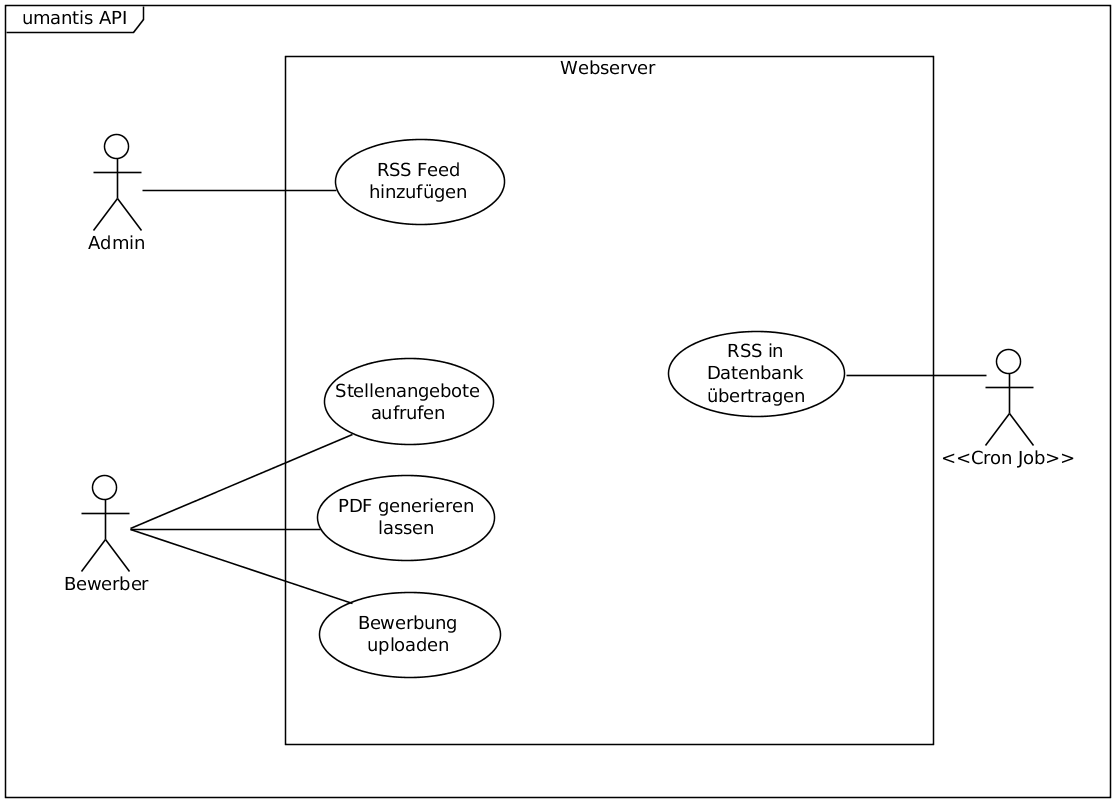
\includegraphics[scale=0.4]{GrobesUseCase}
    \section{Produktfunktionen}
\textbf{/F010/} Cron-Job Einrichtung \\
Auf der Linux Maschine von reality bytes wird ein Cron-Job angelegt, welcher die Funktion /F100/ stündlich aufruft.
\\ \\
\textbf{/F100/} RSS Feed laden und speichern \\
Die im umantis System eingepflegten Stellenangebote werden über einen RSS Feed ausgelesen.
Die enthaltenen Informationen werden in der Datenbank von reality bytes gespeichert.
Bereits enthaltene Einträge werden zur Aktualisierung überschrieben.
Nicht mehr enthaltene Stellenangebote werden aus der Datenbank gelöscht.
\\ \\
\textbf{/F210/} Auslesen der Stellenangebottitel aus der reality bytes Datenbank und Ausgabe \\
Es werden alle Stellenangebottitel ausgelesen und als Übersichtsseite auf der reality bytes Website ausgegeben.
\\ \\
\textbf{/F220/} Auslesen aller Stellenangebotdaten der reality bytes Datenbank und Ausgabe \\
Durch Klicken eines Stellenangebotes auf der Übersichtsseite wird die reality bytes Website neu aufgebaut. Dabei wird eine Detailseite generiert, welche alle Informationen zum gewählten Stellenangebot beinhaltet, was über eine neue Datenbankanfrage erfolgt.
\\ \\
\textbf{/F310/} Generierungsmöglichkeit einer Detailseite zu einer PDF \\
Es wird ein Bibliothek eingesetzt, welche die Funktionalität der Generierung eines Stellenangebots als PDF zur Verfügung stellt. Dieses wird auf der Detailseite der Stellenangebote eingebunden.
\\ \\
\textbf{/F311/} Downloadmöglichkeit der PDF \\
Die abgeschlossene Generierung wird das PDF in einem neuen Tab öffnen, wo es dem \gls{User} möglich ist, das Dokument zu downloaden.
\\ \\
\textbf{/F410/} Implementierung eines Bewerbungsformulars \\
Unter der Detailseite des Stellenangebots wird ein \gls{Button} implementiert, welcher zum Bewerbungsformular weiterleitet. Das Bewerbungsformular beinhaltet die folgenden Eingabefelder für den Bewerber: Vorname, Nachname, Straße, Hausnummer, PLZ, Ort, Telefon, E-Mail, Website, Geburtsdatum, mögliches Eintrittsdatum und eine \gls{Uploadmoeglichkeit} weiterer Dokumente, welche in der Funktion /F430/ näher erläutert wird.
\\ \\
\textbf{/F420/} Validierung des Bewerbungsfomulars \\
Folgende Felder werden im Bewerbungsformular geprüft: Vorname, Nachname, Telefon, E-Mail, Geburtsdatum. Es wird außerdem auf den korrekten Aufbau der E-Mail validiert.
\\ \\
\textbf{/F421/} Fehlerausgaben nach der Validierung \\
Sollte die Validierung fehlschlagen wird unter den betroffenen Eingabefeldern ein Fehlertext ausgegeben. Zusätzlich wird das betroffene Eingabefeld rot umrandet.
\\ \\
\textbf{/F430/} Uploadmöglichkeit von Dokumenten \\
Es können weitere Dokumente vom Bewerber hochgeladen werden mit einer maximalen Dateigröße von 10 Megabyte pro Dokument. Maximal können 5 Dokumente angehängt werden in den Formaten: PDF, ZIP.
\\ \\
\textbf{/F440/} Speichern der Bewerbungsdaten für den umantis Server \\
Die erfassten Bewerbungsdaten werden in XML Format dem umantis System für den Import bereitgestellt.
\\ \\
\textbf{/F450/} Versand einer Informationsmail bei eingehender Bewerbung \\
Nach der Funktion /F440/ wird eine Informationsmail an die Personalabteilung gesendet.

    \section{Produktdaten}

    \textbf{/D10/} Daten der Stellenangebote \\
    ID, Titel, Beschreibung
    \section{Produktleistungen}

Keine besonderen Produktleistungen vorhanden.

    \section{Qualitätsanforderungen}
    Die Qualitätsanforderungen an das Produkt wurden durch den Auftraggeber vorgegeben. Diese beinhalten folgende Punkte:
    \begin{itemize}
        \item Erweiterbarkeit
        \item Übliche Softwarewartung
        \item Benutzerfreundlichkeit
        \item Performance
        \item Stabilität / Zuverlässigkeit
        \item Vollständigkeit
    \end{itemize}
%
    Auf die Erweiterbarkeit wird hohen Wert gelegt. Dies wirkt sich unter anderem auf die anderen Qualitätsmerkmale aus. Außerdem soll es dadurch in Zukunft möglich sein eine Bearbeitung aus einer anderer Hand zu ermöglichen.
    \\ \\
    Die Übliche Softwarewartung zeichnet sich mit kommentierten und strukturierten Quellcode ab. Die Produktfunktionen sollen im Code erkennbar sein.
    \\ \\
    Die Benutzerfreundlichkeit ist ebenfalls wichtig. Der Kunde legt Wert auf eine
    selbsterklärende und intuitive Oberfläche.
    \\ \\
    Durch Performance soll eine angemessene Datenverarbeitungsgeschwindigkeit sichergestellt werden. Diese sollte sich im angemessenen Rahmen befinden, indem keine lange Wartezeiten bei der Verwendung des Produkts auffallen.
    \\ \\
    Unerlässlich ist die Stabilität bzw. Zuverlässigkeit, welche eine stetige Erreichbarkeit unserer Server vorausgesetzt und beim Produkt selber eine niedrige bis keine Fehlertoleranz erzielt.
    \\ \\
    Die Vollständigkeit wird hoch geschätzt, da alle Synergien übereinstimmen müssen, damit die Software erfolgreich verwendet werden kann.

    \section{Benutzeroberfläche}
    Die Benutzeroberfläche soll durch die zur Verfügung gestellten Schnittstellen dieses Produktes frei gestalterisch ermöglicht werden. Ein spezifisches Design ist hier nicht gewünscht. Ein schlichtes Formular, mit Eingabefeldern zur Person, ein Upload Button für weitere Bewerbungsunterlagen, ein Absendebutton und die Möglichkeit die Bewerbung in PDF zu konvertieren sollten gegeben sein.

    \section{Nichtfunktionale Anforderungen}

    Es wird ein plattformunabhängiges Produkt entwickelt, welches über jeden aktuellen Browser erreichbar sein wird.
    \section{Technische Produktumgebung}

    Das Produkt ist eine Client/Serveranwendung, genauer gesagt eine Webbrowseranwendung.

    \subsection{Software}

    \textbf{Server:}
    - OS: Linux Debian ab Version 4.3.5
    - Webserver Apache ab Version 2.2
    - PHP ab Version 5.3.3
    - MySQL ab Version 5.1

    \textbf{Client:}
    - Beliebige PC-Hardware
    - Intranet-Zugang
    - Aktuelle Browserversion
    - Javascript

    \subsection{Hardware:}

    \textbf{Server:}
    - Standardhardware
    - Netzwerkfähig

    \textbf{Client:}
    - Standardhardware
    - Netzwerkfähig

    \subsection{Orgware:}
    Keine

    \subsection{Produkt-Schnittstellen}
    Für die Entwicklung wären keine gesonderten Schnittstellen zu nennen, da unter anderem PHP nicht kompiliert werden muss.
    \section{Spezielle Anforderungen an die Entwicklungs-Umgebung}

    \subsection{Software}

    - Betriebssystem: Linux Mint 17.3 Rosa
    - IDE: Lizensiertes PhpStorm 10.0.2

    \subsection{Hardware}
    - Standart PC

    \subsection{Orgware}
    - Netzwerkverbindung

    \subsection{Entwicklungs-Schnittstellen}
    Die Entwicklungsumgebung ist nur dafür gedacht um Code zu generieren und zu überprüfen,
    die Interpretation findet im Browser statt. Wenn der Code erfolgreich auf Syntaxfehler
    getestet wurde, wird auf dem Entwicklungsrechner auf die Funktionalität geprüft.
    \section{Gliederung in Teilprodukte}

    Es gibt keine Unterteilung in Teilprojekte.
    \section{Ergänzungen}

    Das Produkt ist ausschliesslich Webbasiert. Das Layout ist nicht an die reality bytes medien GmbH einer bestimmen Einrichtung angepasst.

\printglossary[title=Glossar, toctitle=Glossar]

\itab{} \\
\itab{------------------------------------} \tab{------------------------------------} \\
\itab{Eduard Luft} \tab{Burkhard Theß} \\
\itab{Unterschrift und Datum} \tab{Unterschrift und Datum} \\



\end{document}
